\section{Testing and evaluation}\label{sec:testing_and_evaluation}
In this next section, we are going to evaluate the performance of the PassGAN system on the Libero set, as well as give a brief overview of our methodology and the experimental setup.

\subsection{Experimental setup}
Both training of the GAN and testing were carried out on a Linux machine running Debian stretch, equipped with a GTX 1070 graphics card, an i5-2500 CPU and 8 GB of system memory. 
With this card, training of PassGAN took roughly twelve hours.
PassGAN was run on Python 2.7, running Tensorflow 1.12.0.%\\

For testing we used the latest stable version of HashCat available at the time (version 5.1.0). %and we observed a peak speed between 850 and 860MH/s (for reference, 1MH/s is equivalent to 1 million candidate passwords hashed and compared per second) %Reference  %The definition of MH is probably wrong

%change position of NL box and make legen entry for optional things green
Figure \ref{fig:testing_flowchart} below illustrates our overall process, which is divided in two Phases: 
\begin{itemize}
    \item A Training Phase, in which we train PassGAN on a given dataset and sample password candidates from the trained model.
    \item A Testing Phase, in which we use HashCat to try and crack a sub-set of the passwords in the libero leak.
\end{itemize}

\begin{figure}[H]
\centering
    \includegraphics[scale=0.7]{figures/testing_flowchart_ocd.png}
    \caption{A diagram illustrating our general workflow for evaluating PassGAN, including Training and Testing}
    \label{fig:testing_flowchart}
\end{figure}    

\subsection{Training the PassGAN system}\label{subsec:passgan-training}
As we explained back in section \ref{subsubsec:gans-passgan}, in order to train PassGAN we took the plain text passwords from the libero leak (667,714 passwords) and split them into two groups. 80\% of the passwords went into our Training Set, while the remaining 20\% of passwords went in the Testing set: the Training set is used to train PassGAN as can be seen in Step 1 of Figure \ref{fig:testing_flowchart}, while the passwords in the Testing set are hashed with MD5 to serve as a cracking target for HashCat as seen in Step 2 of figure \ref{fig:testing_flowchart}. We will go into further detail with the Testing set in section \ref{subsec:passgan-testing}, as the brief explanation provided here is not entirely accurate.

PassGAN can additionally be trained on Natural Language data, shown in a dotted box in figure \ref{fig:testing_flowchart}; elements shown within a dotted box are considered optional, they can be included or not. Natural Language data will be further discussed in section \ref{subsec:nl-testing}.

Once PassGAN is done training with a given dataset, it produces a trained model that can be used to generate candidate passwords via sampling (Step 1.1 in figure \ref{fig:testing_flowchart}).\\ 
We covered the concept of models back in section \ref{subsubsec:gans-passgan}, but as a reminder a model is a snap-shot of the internal state of a network, containing all the weights and parameters necessary to process new input (or generate password candidates with the features learned from the training data, in the case of PassGAN).

We can use the trained model produced at the end of training to sample password candidates generated from PassGAN: The result of the sampling process will be a list of candidate passwords that make up the PassGAN wordlist used with HashCat when testing. We can choose to generate more or less candidate passwords when sampling: the tests listed in table \ref{tab:test-set} use a wordlist of 1 million password candidates, while tables \ref{tab:passgan-big} and \ref{tab:nl-results} use a wordlist of roughly 14 million password candidates.


%In order to train the PassGAN system, we extracted the plain text passwords from the original file (which was formatted in JSON as it contained personal information beyond just the emails and passwords of the users), and split it up in two sets: a training set containing 80\% of the passwords (534,171 entries) and a testing set containing 20\% of the passwords (133,542 entries).
%We used the model trained on the bigger set to generate 1 million samples from PassGAN, that then served as the basis from our initial testing.

Below is a small sample of password candidates generated by PassGAN, taken from the 1 million wordlist: %Maybe i should take a sample from the last checkpoint instead?
\begin{verbatim}
22052906    mariamuna   iaup63     poldetta53
001178      04051987    topolapa    aenara
rotsanera   princone    fadyreda21  giugki
dimonepa72  12orlomon   deb57828    belnabola
marcanalla  ACADCNAN   leegenniki  vicaletto
\end{verbatim}

%Give a small example of one or two particular words and words in italian that resemble them.
What we found particularly interesting was that while the samples showed the typical patterns exhibited by user-generated passwords (numbers appended or pre-pended to words, so-called leet speak etc..), a majority of them also seemed to mimic Italian words and phrases: most of these words were meaningless, but nonetheless we speculated that the GAN might be trying to \enquote{learn} Italian as a side-effect of generating samples close to the input data distribution.
As an example the string \texttt{vicaletto} resemble the italian word \enquote{vicoletto} meaning \enquote{a narrow street}, while the string \texttt{princone} sounds vaguely like the italian word for pickaxe, \enquote{piccone}. 

\subsection{Testing the PassGAN system}\label{subsec:passgan-testing}

\begin{figure}[H]
\centering
    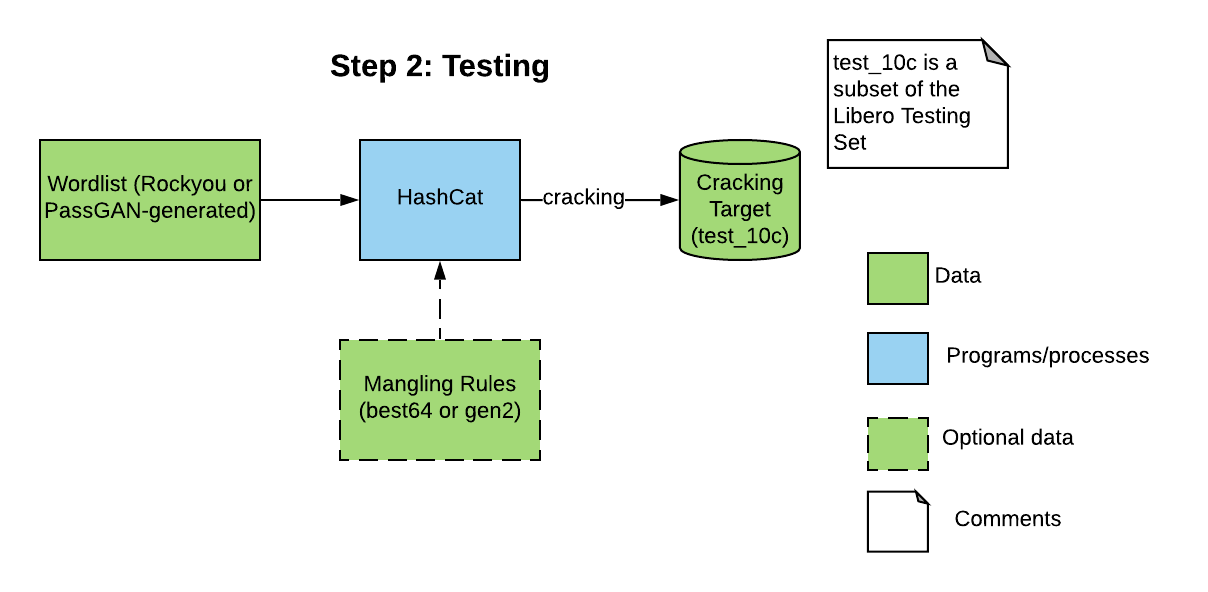
\includegraphics[scale=0.8]{figures/testing_only.png}
    \caption{A zoomed-in version on the previous diagram, showing only the Testing process}
    \label{fig:testing_only}
\end{figure}    

The testing process is depicted in figure \ref{fig:testing_only}: In it we use HashCat to crack a sub-set of the Libero leak passwords (the cracking target), using a wordlist and optionally a set of mangling rules as input.

%This section is still convoluted
The cracking target is a sub-set of the Libero Testing set, that itself is a set of 20\% of the libero leak passwords that we set aside from testing as mentioned in the very beginning of section \ref{subsec:passgan-training}.
% make it more clear that we are copying the passgan paper.
Our cracking target is not the whole Testing set, but a sub-set of it composed of passwords with a length of 10 characters or less: this was done because Hitaj. et al. \cite{PassGAN} also limit their testing with HashCat in this same way, we decided to do it too in order to more closely follow their methodology; as to the reason why this limitation is in place, we speculate this is done to better suit the passwords in the cracking target to PassGAN. As we mentioned back in section \ref{subsubsec:gans-passgan}, PassGAN sets the \emph{Sequence Length} hyper-parameter to 10 during training: this parameter sets the maximum length of password candidates generated by PassGAN during sampling, so testing against a sub-set of 10-character passwords is a way to tailor the cracking target to PassGAn's output slightly.
We do not fully understand why Hitaj. et al. made this choice, but nonetheless we adopted it ourselves in an effort to more closely mimic their evaluation process.

We believe this sub-set of ten character passwords still represents the whole Testing set fairly, as not many passwords were removed: the vast majority of passwords in the Testing set are 10 characters or less, 111,994 or 83.86\% to be precise. 
From here on, we will refer to this sub-set of 10 character passwords as \emph{test\_10c} (the actual filename) or more simply as \enquote{the cracking target}

% During our testing we tried to follow the same sort of methodology that Hitaj et al.\cite{PassGAN} used in their paper: as such our cracking target is not the whole Testing set, a sub-set of it composed of passwords with a length of 10 characters or less: This was done to better use PassGAN, as during training we set the maximum sequence length to 10.
% We believe this sub-set of ten character passwords still represents the whole Testing set fairly, as not many passwords were removed: the vast majority of passwords in the Testing set are 10 characters or less, 111,994 or 83.86\% to be precise. 
% From here on, we will refer to this sub-set of 10 character passwords as \emph{test\_10c} (the actual filename) or more simply as \enquote{the cracking target}

Touching upon the wordlist and rules used, they are also depicted in figure \ref{fig:testing_flowchart}: for the former we use either the \emph{RockYou} wordlist or a wordlist generated by PassGAN, while for the latter we use either the \emph{best64} or \emph{generated2} rule sets. Both the RockYou wordlist and the two rulesets mentioned above were chosen because they were used in Hitaj et al. \cite{PassGAN}, but also because they are widely used and understood to be among the more efficient wordlists available to an attacker. We believe that they demonstrate rather well what rule-based password crackers can do without further language specific optimizations such as those that PassGAN provides. %Reference, nigga

The RockYou wordlist contains more than 14 million passwords, all of which come from various data breaches that have been compiled into one resource; it contains password of varying length and complexity, and as such should provide a good performance baseline for rule-based crackers. The best64 rules file contains around 70 mangling rules, while the genrated2 rules file contains more than 65,000. 

The tables below will illustrate the results of our tests attacking the cracking target with different combination of Wordlists and rules. To clarify, we decided early on to use mangling rules also when testing password samples from PassGAN, since they greatly increased the number of passwords found compared to just using a wordlist. 
To the best of our understanding Hitaj. et al. have not used rules in their evaluation of PassGAN, but instead have chosen to generate a huge number of password candidates and use PassGAN alone to match passwords in the cracking target. We have also briefly tried this approach, our experience with it will be detailed in section \ref{subsubsec:huge-wordlists}}%If you wanna put the results for huge passgan wordlist here is where they go
%This is not something that Hitaji and al. seem to have done, they seem to have used only PassGAN-generated wordlist to crack their target db. We tried and we got really shit results

As a final note, HashCat's default behaviour is to cache passwords found during an attack in what the HashCat manual calls a \emph{potfile}, so that if an attacker chooses to approach the target using a different wordlist or a different set of rules, no time is wasted cracking passwords that were already found previously; because using different rule sets can greatly affect the efficiency of cracking, this form of caching allow an attacker to crack more passwords by combining different approaches.
In order to test the performance of each wordlist and rule combination separately, we disabled caching of cracked passwords between cracking attempts: this was done with the HashCat command showed in the code snippet in section \ref{sec:libero}, and it allowed us to evaluate the performance of different combination of wordlists and rules singularly. However disabling the potfile also leads to a lower overall number of passwords found. Tables \ref{tab:test-set}, and \ref{tab:passgan-big} show show tests done with caching disabled, while the figures obtainable with caching will be mentioned in section \ref{subsubsec:potfile-enable}. 

\begin{table}[H]
\begin{tabular}{|l|c|c|c|}
\hline
\textbf{\emph{Wordlist/Ruleset}} & \textbf{-} & \textbf{Best64} & \textbf{Generated2} \\ \hline
\textbf{Rockyou}          & 19,215 (23.78\%) & 30,170 (37.33\%) & 59,134 (73.18\%) \\ \hline
\textbf{PassGAN}          & 4,637 (5.74\%) & 11,053 (13.68\%) & 34,896 (43.18\%) \\ \hline
\end{tabular}
\caption{A comparison of the number of passwords found in the cracking target by RockYou and PassGAN,  using a 1 million wordlist for PassGAN}
\label{tab:test-set}
\wfill
\hfill
\end{table}

Table \ref{tab:test-set} shows that PassGAN performs rather poorly in comparison with the RockYou wordlist: we attributed this shortcoming to two main factors: firstly the size of the wordlist generated by PassGAN, which is 1 million entries as opposed to the 14+ million entries of RockYou, and secondly the quality of the PassGAN wordlist. Both of these factors play into each other, because while the rules provide great advantages in terms of password found, ultimately they just modify the entries in the wordlist. Thus we might say that the whole system is limited by the capabilities of the wordlist that is used.

In order to test this hypothesis we used our existing PassGAN model to generate a bigger wordlist with as many entries as as RockYou, and performed a second test:
\begin{table}[H]
\centering    
\begin{tabular}{|l|c|c|c|}
\hline
\textbf{\emph{Wordlist/Ruleset}} & \textbf{-} & \textbf{Best64} & \textbf{Generated2} \\ \hline
\textbf{Rockyou}          & 19,215 (23.78\%) & 30,170 (37.33\%) & 59,134 (73.18\%) \\ \hline
\textbf{PassGAN}          &  10,735 (13.28\%) & 20,638 (25.54\%) & 48,751 (60.33\%) \\ \hline
\end{tabular}
\caption{A comparison of the number of passwords in the cracking target found by RockYou and PassGAN, using a 14 million wordlist for PassGAN} 
\label{tab:passgan-big}
\end{table}

As table \ref{tab:passgan-big} shows, PassGAN found roughly 15\% more passwords when using a bigger wordlist: this leads us to believe that wordlist size and quality does constitute a performance bottle-neck. It should be also noted that when compared with the original, 1 million string wordlist, we found a significant 40\% overlap in the strings that were generated. Addressing the problem of quality of the wordlist, we speculated that one of the reasons for the gap in efficiency between PassGAN and RockYou might be the fact that the strings generated by PassGAN don't follow grammatical rules, and this might have hindered the efficacy of the base wordlist. This hypothesis however was later proven wrong by our natural language experiments, detailed in section \ref{subsec:nl-testing}
%Talk about the 50mil and 100mil exapriements

\subsubsection{Running HashCat with caching}\label{subsubsec:potfile-enable}
Now that we had an idea of the performance of each method, we wanted to see what was the maximum number of passwords we could find by combining the two approaches (RockYou and PassGAN):
In order to do this we took the best performing ruleset (generated2), and we performed two rounds of cracking with caching enabled. First we run RockYou with the generated2 ruleset, that yielded the same results shown in Table \ref{tab:passgan-big} for that particular combination; next we tried PassGAN plus generated2, which yielded a final result of 63,847 passwords found (79.01\% of the cracking target). Running the two approaches in combination seems to definitely be more affective that using PassGAN alone, as there are many passwords that PassGAN cannot find but that are cracked by the RockYou wordlist.
Furthermore when we look at the two lists of cracked passwords, we can notice around 5,000 unique passwords that were matched by PassGAN but not Rockyou, showing that PassGAN might have some potential as a tool to close in on more difficult passwords that have a specific linguistic provenance. Looking at some of these unique passwords, they mostly consist of proper names and more obscure italian words.

\subsubsection{Testing the limits of PassGAN wordlist size}\label{subsubsec:huge-wordlists}
As we said previously Hitaj. et al. \cite{PassGAN} don't seem to have used rules when testing PassGAN: instead they seem to have taken a different approach, taking advantage of the fact that PassGAN can generate arbitrary numbers of password candidates from a trained model; these password candidates may not match the target as well as the passwords in an established wordlist like RockYou, but PassGAN can generate vast quantities of them: thus Hitaj. et al chose a \enquote{quantity over quality} approach.

We were interested in seeing how such huge wordlists would perform without the help of rules, so we run a couple of tests: we took our existing PassGAN model, our standard cracking target \texttt{test\_10c}, and we generated three new wordlist for PassGAN: one with 50 million entries, one with 100 million entries And finally one with roughly 196 million entries. 
The reason why we chose these 3 steps is simple: as we can see in tables \ref{tab:test-set} and \ref{tab:passgan-big}, going from 1 million entries to 14 million entries yielded 15\% more passwords, so we wanted to see if testing a wordlist with $14^2$ million passwords would yield roughly 15\% more results compared with table \ref{tab:passgan-big}. The 50 million and 100 million wordlists are intermediate steps that can give us clues on how the number of passwords scales with wordlist size.
%The 50 million wordlist managed to crack 13.898 passwords (17.20\% of the cracking target), while the 100 million wordlist managed to crack 15.669 passwords (19.39\% of the target).\\
%While the increase between the two
\begin{table}[H]
\centering    
\begin{tabular}{|l|c|c|c|}
\hline
\textbf{\emph{Wordlist/Ruleset}} & \textbf{-} & \textbf{Best64} & \textbf{Generated2} \\ \hline
\textbf{PassGAN (50 million passwords)}          & 13.898 (17.20\%) & - & - \\ \hline
\textbf{PassGAN (100 million passwords)}          & 15.669 (19.39\%) & - & - \\ \hline
\textbf{PassGAN (200 million passwords)}          & 17.523 (21.68i\%) & - & - \\ \hline
\end{tabular}
\caption{A comparison of the number of passwords found by just PassGAN using different wordlist sizes and no mangling rules} 
\label{tab:passgan-big}
\end{table}

\subsection{Training PassGAN with Natural Language corpora} \label{subsec:nl-testing}
%Find a more reader-friendly explanation for grammatical correctness, especially at the beginning  when defining the goal.
Our next step was to include natural language data in the input and re-train the model, in the hope that this new input data would help the system generate more grammatically correct strings and thus improve the number of passwords matched.

Firstly though we should define what our goal was for using Natural Language with PassGAN, and what we mean with grammatical correctness. 
As we showed at the end of section \ref{subsec:passgan-training}, a sizeable number of the password candidates generated by PassGAN during sampling are words: in the context of the strings generated by PassGAN, we define a \enquote{word} as simply a string composed of uppercase and/or lowercase letters. It might be entirely composed of letters like the two examples we gave in section \ref{subsec:passgan-training}, or have numbers pre-pended or appended to it. As we mentioned in those examples, most of the words generated by PassGAN when trained on passwords exclusively are meaningless: they may resemble italian words, but they are ultimately incorrect.
%whats wrong with saying grammatical correctness is that peple may think about sentences adn passphrases
Our goal for training PassGAN with natural language data was to hopefully teach the system enough about the italian language to turn a decent part of those meaningless words into actual italian words. In Turn, we thought, that might have yielded better results in terms of number of password cracked and especially in terms of their quality: We hoped the inclusion of Natural Language data would allow us to match more language-specific passwords like those 5,000 unique passwords mentioned in \ref{subsubsec:potfile-enable}   

% the two corpoora were put toghether by other people, i simpl sampled them.
% say that and cite sources
%Maybe put an excract from the 2 corpora in here too.
For this purpose we have chosen two different corpora of Italian Natural Language samples: 
\begin{itemize}
    \item The Repubblica corpus: A corpus of words extracted from the italian newspaper \enquote{Repubblica}, taken from articles published between 1985 and 2000 (roughly 380 million words).\cite{repubblica_corpus}
    \item The ItWaC corpus: A large 2 billion word corpus obtained by crawling internet sites under the \texttt{.it} domain. \cite{itwac_corpus}.  
\end{itemize}

%You can increase the number of guesses by generating more samples and increasing the size of the wordlist, though there might be diminishing returns at some point.
%The nice thing about PassGAN is that you have theoretically infinite wordlists, even if the quality might be up and down.
Both corpora were generated using the NoSketch Engine online tool \cite{nosketch_engine}, and we decided to sample one dataset from each corpus with the same number of entries as the libero password set: we sampled 700,000 words from both the Repubblica corpus and the ItWac corpus, and those two files served as the basis for our Training. This was done to ease the process of organizing data for training PassGAN, and also because we were interested the impact that different ratios of password data to natural language data might have on the resulting model.
Previous research \cite{Melicher2016} has suggested that introducing Natural Language data into a system trained on passwords tends to generate a lot of noise during training, and our results turned out to be in line with that paper.

Both corpora were simply a list of italian words, ranked by their frequency in the corpus: the file produced by the NoSkecth tool has a list of words in descending frequency and their frequency count.
In order to prepare the data for training, went through a similar process to what we did for the libero leak passwords: we divided each corpus into an 80\%-20\% (we realized later this step was entirely unnecessary, as we had no intention of using NL data as a cracking target) and then proceeded to make two wordlist out of each natural language corpus.

The shell commands we used to accomplish this are shown below:

\begin{lstlisting}[language=bash,numbers=left,stepnumber=1,breaklines=true,postbreak=\mbox{\textcolor{red}{$\hookrightarrow$}\space}]
#Split each NL corpus into 80%-20% (not strictly necessary)
head -n 534172 Repubblica_700k.txt|cut -f1 > Repubblica-80.txt
tail -n 133543 Repubblica_700k.txt|cut -f1 > Repubblica-20.txt

head -n 534172 ItWac_700k.txt|cut -f2 > ItWac_80.txt
tail -n 133543 ItWac_700k.txt|cut -f1 > ItWac_20.txt

#Create training data for PassGAN with password data + 50% of the Repubblica corpus
shuf -n 267086 Repubblica-80.txt|cat - ../libero\ it\ July\ 2016/train.txt|shuf > libero+Repubblica-50.txt

#Create training data for PassGAN with password data + 100% of the repubblica corpus
shuf Repubblica-80.txt|cat - ../libero\ it\ July\ 2016/train.txt|shuf > libero+Repubblica.txt

#Create training data for PassGAN with password data + 50% of the ItWaC corpus
shuf -n 267086 ItWac_80.txt|cat - ../libero\ it\ July\ 2016/train.txt|shuf > libero+ItWac-50.txt

#Create training data for PassGAN with password data + 100% of the ItwaC corpus
shuf ItWac_80.txt|cat - ../libero\ it\ July\ 2016/train.txt|shuf > libero+ItWac.txt
\end{lstlisting}

As we can see in the code snippet above, we created two training datasets for each corpus: one contained all the passwords in the Libero Training set and 50\% of the Natural language data, while the other contained all of the Training set passwords and all of the Natural Language data: we did this because we wanted to see what impact different amounts of natural language data had on PassGAN's performance (if any).

We thus proceeded to train 4 separate instances of PassGAN with our four datasets, and then sampled each trained model for testing: the results were 4 separate wordlists, each of around 14 million entries, that we used in HasCat to attack the same cracking target that we used in the previous section (test\_10c).

Touching upon the impact of NL data on the model performance, our hypothesis was that we might see a decrease in model performance when training with 100\% of the natural language data since each corpus contains as much data as the Libero Training set; By combining the two into a single dataset for training, we effectively use as much NL data as password data.  We though this might lead to noise and ‘confuse’ PassGAN, resulting in a model with less focus on generating passwords and more focused on generating NL samples. While that is technically true, overall table \ref{tab:nl-results} shows that the introduction of NL data does not seem to have any noteworthy impact on cracking performance.

The results of our tests on all four wordlists are shown in table \ref{tab:nl-results} below.

\begin{table}[H]
\centering
\begin{tabular}{|l|c|c|c|}
\hline
 \textbf{\emph{Wordlist/Ruleset}} & \textbf{-} & \textbf{Best64} & \textbf{Gen2} \\ \hline
 \textbf{Libero+Repubblica 50\%} & - & - & 51,232 (63.40\%) \\ \hline
 \textbf{Libero+Repubblica 100\%} & - & - &  48,651 (60.20\%) \\ \hline
 \textbf{Libero+ItwaC 50\%} & - & - &  50,133 (62.04\%) \\ \hline
 \textbf{Libero+ItWaC 100\%} & - & - &  47,646 (58.96\%) \\ \hline
\end{tabular}
\caption{Number of passwords found using PassGAN, trained on passwords and Natural Language data}
\label{tab:nl-results}
\end{table}

As we can see the results of training with natural language data are very similar to just using PassGAN+gen2 as shown in table \ref{tab:passgan-big}; there is a slight improvement of 2-3\% when using the datasets containing 50\% of language data, but we do not believe it is a significant change. This result seems to be in line with Melicher et al.\cite{Melicher2016}, and it seems to show us that natural language data does not have much of an impact on the output of PassGAN. 
%\newpage
If we take a random sample from the Repubblica 50\% set, the one that performed the best even if marginally so, we can see that there has not been a substantial improvement in the grammatical correctness of the words in the sample.:
\begin{verbatim}
c3b243dc    fetemanio   carcilla    RATS1203
valentto    itefis82    carmoinx    gip1904
sederonco   elestarsia  220689      QunkYYTx84
n!utelo     kedea       Colpudari   rich1770
aletsa      simoshero   gidni12     1uva1[78
\end{verbatim}    

The words that PassGAN generates are still meaningless and do not seem to have a higher degree of grammatical correctness, the only change we have been able to observe is in the fact that more strings seem to be composed of letters exclusively.

This does not discredit the use of Natural language as a whole, but points us toward the fact that natural language generation and password generation might two different workloads that may not be accomplished well with the same machine learning system: it seems that introducing Natural Language data into PassGAN simply adds noise to the system and does not contribute to the system's performance.
The results in table \ref{tab:nl-results} and the effectiveness of mangling rules as a cracking tool also hint at the idea that user-generated passwords may be defined by their patterns more than by their language of origin.
